\documentclass{article}
\usepackage{amsmath,amssymb,graphicx}
\usepackage[margin=1in]{geometry}
\usepackage[colorlinks=true,linkcolor=blue,urlcolor=blue]{hyperref}

\newcommand{\Tg}{T_\gamma}
\newcommand{\Mpl}{M_{\mathrm{Pl}}}
\newcommand{\Ggg}{\Gamma_{\phi\to\gamma\gamma}}
\newcommand{\Ds}{\mathcal{D}}

\title{$\gamma\gamma\to\phi\phi$: cross section, and when it beats inverse decay}
\date{}
\begin{document}\maketitle

\noindent\fbox{\parbox{\dimexpr\linewidth-2\fboxsep}{\small
\textbf{Superseded for S$\otimes$S and P$\otimes$S (2026-10-22).} For a scalar
$\phi$ coupled to quark masses, $\gamma\gamma\to\phi\phi$ is dominated by the
charged-meson loop itself (boxes plus seagull triangle), not by the photon
exchange computed here: see \texttt{notes/gg\_phiphi\_box.tex},
$\sigma=\alpha^2Y^2s\beta/(36864\pi^3)$, about $10^7$ times larger.
\texttt{neff\_simple} uses that for S$\otimes$S/P$\otimes$S and keeps the
photon exchange below only for the other models.}}


\section{The vertex, normalised to $\Ggg$}

The only $\phi$--photon coupling in this model is the loop-induced operator
%
\begin{equation}
  \mathcal{L} = \frac{g_{\phi\gamma\gamma}}{4}\,\phi\,F_{\mu\nu}F^{\mu\nu},
  \qquad
  V^{\mu\nu}(a,b) = i\,g_{\phi\gamma\gamma}\big[(a\!\cdot\! b)\,g^{\mu\nu} - b^\mu a^\nu\big],
  \label{eq:vertex}
\end{equation}
%
with both photon momenta incoming. It is transverse in each index,
$a_\mu V^{\mu\nu}=0$, so Feynman gauge may be used for internal photons.
Squaring it for the decay gives $\sum_{\rm pol}|\mathcal{M}|^2 =
g_{\phi\gamma\gamma}^2 m_\phi^4/2$ and hence
%
\begin{equation}
  \Ggg = \frac{g_{\phi\gamma\gamma}^2 m_\phi^3}{64\pi}
  \qquad\Longrightarrow\qquad
  g_{\phi\gamma\gamma}^2 = \frac{64\pi\,\Ggg}{m_\phi^3}
  = \frac{\alpha^2\Ds}{72\pi^2},
  \label{eq:gnorm}
\end{equation}
%
the last equality using \texttt{phi\_partial\_widths.m},
$\Ggg=\alpha^2\Ds m_\phi^3/(4608\pi^3)$. \emph{The coupling is
$m_\phi$-independent}: for $g=[1\,1\,1]/3$, $\Ds=1.86\times10^5\,$GeV$^{-2}$
and $g_{\phi\gamma\gamma}=1/(8.48\,\mathrm{GeV})$. Everything below follows
from eq.~\eqref{eq:vertex} alone, so it is fixed by $\Ggg$ with no new
parameter.

\section{Amplitude}

With a $\phi\gamma\gamma$ vertex and no $\phi^2\gamma\gamma$ seagull, the only
tree topologies for $\gamma(k_1)\gamma(k_2)\to\phi(p_1)\phi(p_2)$ are
$t$- and $u$-channel \emph{photon} exchange, two insertions of
eq.~\eqref{eq:vertex}:
%
\begin{equation}
  \mathcal{M} = \frac{i\,g_{\phi\gamma\gamma}^2}{t}\,
    \epsilon_{1\mu}\epsilon_{2\nu}B^{\mu\nu}(k_1,k_2;q_t)
  \;+\;(k_1\leftrightarrow k_2,\ t\to u),
  \qquad q_t = p_1-k_1,\quad t=q_t^2,
\end{equation}
%
\begin{equation}
  B^{\mu\nu}= -(k_1\!\cdot\! q)(q\!\cdot\! k_2)g^{\mu\nu}
   + (k_1\!\cdot\! q)k_2^\mu q^\nu + (q\!\cdot\! k_2)q^\mu k_1^\nu
   - (k_1\!\cdot\! k_2)q^\mu q^\nu .
\end{equation}
%
Each vertex carries two powers of momentum and the propagator one inverse
power, so $\mathcal{M}\sim g_{\phi\gamma\gamma}^2 s$: the amplitude
\emph{grows} with energy, and carries no $m_\phi$ suppression.

\section{Squared amplitude}

Averaging over the four initial linear-polarisation combinations,
%
\begin{equation}
  \overline{|\mathcal{M}|^2}
  = \frac{g_{\phi\gamma\gamma}^4\,s^2}{32}\,\frac{N(c)}{\big[s^2\beta^2(1-c^2)+4m_\phi^4\big]^2},
  \qquad
  \beta=\sqrt{1-\frac{4m_\phi^2}{s}},\quad c=\cos\theta,
  \label{eq:Msq}
\end{equation}
%
\begin{equation}
  N(c) = A_4\,(1-c^2)^2 + 32\,m_\phi^4 s^2\beta^2\,(1-c^2) + 64\,m_\phi^8,
\end{equation}
\begin{equation}
  A_4 = 5s^4 - 44m_\phi^2 s^3 + 116 m_\phi^4 s^2 - 96 m_\phi^6 s + 64 m_\phi^8 .
\end{equation}
%
The denominator is just the two propagators: $s^2\beta^2(1-c^2)+4m_\phi^4 = 4tu$
identically, with $t,u = m_\phi^2 - \tfrac{s}{2}(1\mp\beta c)$. It never
vanishes for physical $c$, since $tu\ge m_\phi^4>0$.

\section{Cross section}

The angular integral is elementary in $x=1-c^2$; the two structures
$\int_{-1}^{1}\!dc\,(\alpha-Ac^2)^{-2}$ and its $c^2,c^4$ partners produce
$\mathrm{artanh}\big(s\beta/(s-2m_\phi^2)\big)$, and since
$(s-2m_\phi^2)^2-(s\beta)^2=4m_\phi^4$ this is
%
\begin{equation}
  L \equiv \mathrm{artanh}\!\left(\frac{s\beta}{s-2m_\phi^2}\right)
    = \ln\!\left(\frac{s-2m_\phi^2+s\beta}{2m_\phi^2}\right).
\end{equation}
%
With $\sigma = \dfrac{\beta}{64\pi s}\displaystyle\int_{-1}^{1}\!dc\,
\overline{|\mathcal{M}|^2}$ (the $\tfrac12$ for identical final-state $\phi$'s
included),
%
\begin{equation}
\boxed{\;
\begin{split}
  \sigma_{\gamma\gamma\to\phi\phi}(s) = \frac{g_{\phi\gamma\gamma}^{4}}{1024\pi}\Bigg[\,
    &\frac{\beta\left(5s^{2}-4m_\phi^{2}s+6m_\phi^{4}\right)}{s} \\[2pt]
    &- \frac{8\,m_\phi^{4}\,(s-3m_\phi^{2})(s-m_\phi^{2})}{s^{2}\,(s-2m_\phi^{2})}\,
      L
  \Bigg]\;
\end{split}}
  \label{eq:sigma}
\end{equation}
%
with limits
%
\begin{equation}
  \sigma \;\xrightarrow[s\to4m_\phi^2]{}\;
  \frac{g_{\phi\gamma\gamma}^{4}m_\phi^{2}\beta}{64\pi}
  = \frac{64\pi\,\Ggg^{2}}{m_\phi^{4}}\,\beta,
  \qquad
  \sigma \;\xrightarrow[s\gg m_\phi^2]{}\;
  \frac{5g_{\phi\gamma\gamma}^{4}s}{1024\pi}
  = \frac{20\pi\,\Ggg^{2}s}{m_\phi^{6}} .
  \label{eq:limits}
\end{equation}
%
Equation~\eqref{eq:sigma} is the expression circulated in the draft; it is
confirmed here. Note the high-energy form is $\sigma\simeq
5s/(1024\pi\Lambda^4)$ with $\Lambda=1/g_{\phi\gamma\gamma}=8.5\,$GeV: the EFT
is valid throughout the BBN-era range used below ($\sqrt{s}\sim T\lesssim
10\,$MeV), and $\sigma$ is independent of $m_\phi$ there.

\subsection*{Verification}

Two independent numerical routes agree with eq.~\eqref{eq:sigma} to 8--9
significant figures over $4\le s/m_\phi^2\le10^6$:
(i) explicit helicity sum of $\mathcal{M}$ with numerical 4-vectors and
Gauss--Legendre angular integration; (ii) numerical integration of the
symbolic $\overline{|\mathcal{M}|^2}$, eq.~\eqref{eq:Msq}. The high-energy
coefficient comes out $4.99999$ vs.\ 5, and the threshold limit matches
eq.~\eqref{eq:limits}. (A symbolic \texttt{integrate} of eq.~\eqref{eq:Msq}
silently drops the $L$ term and returns only the first line of
eq.~\eqref{eq:sigma}; that output is wrong, as the numerics show.)

\section{Comparison with the inverse-decay portal}

\texttt{neff\_dark.m} takes the SM$\leftrightarrow$dark portal rate as
$\max[R_{\gamma\gamma\to\chi\chi}/n_\gamma,\ \Ggg K_1/K_2]$. The pair-production
channel $\gamma\gamma\to\phi\phi$ is absent. Its thermal rate, in the same
Gondolo--Gelmini normalisation,
%
\begin{equation}
  \Gamma_{\gamma\gamma\to\phi\phi}
  = \frac{1}{n_\gamma}\frac{\Tg}{16\pi^4}\int_{4m_\phi^2}^{\infty}\!\!ds\,
    \sigma_{\gamma\gamma\to\phi\phi}(s)\,s^{3/2}K_1(\sqrt{s}/\Tg)
  \;\xrightarrow[\Tg\gg m_\phi]{}\;
  127\,\frac{\Ggg^{2}\,\Tg^{5}}{m_\phi^{6}},
\end{equation}
%
using $\int_0^\infty\!u^6K_1(u)du=384$, while the inverse-decay branch falls,
$\Ggg K_1/K_2 \to \Ggg m_\phi/2\Tg$. Hence
%
\begin{equation}
  \frac{\Gamma_{\gamma\gamma\to\phi\phi}}{\Ggg K_1/K_2}
  = 254\,\frac{\Ggg\,\Tg^{6}}{m_\phi^{7}},
  \qquad
  T_* = m_\phi\left(\frac{m_\phi}{254\,\Ggg}\right)^{1/6}
      = \left(\frac{1.06\times10^{7}\,m_\phi^{4}}{\Ds}\right)^{1/6}
      \simeq 1.97\,m_\phi^{2/3}\ \mathrm{GeV},
  \label{eq:Tstar}
\end{equation}
%
the last form for $g=[1\,1\,1]/3$. Inverse decay dominates only below $T_*$.
The reason is structural: inverse decay is suppressed by $m_\phi^3$ in $\Ggg$
\emph{and} again by $K_1/K_2\simeq m_\phi/2\Tg$, whereas pair production runs
on the same operator at $\sqrt{s}\sim\Tg$ with no $m_\phi$ suppression at all.

\begin{figure}[h]\centering
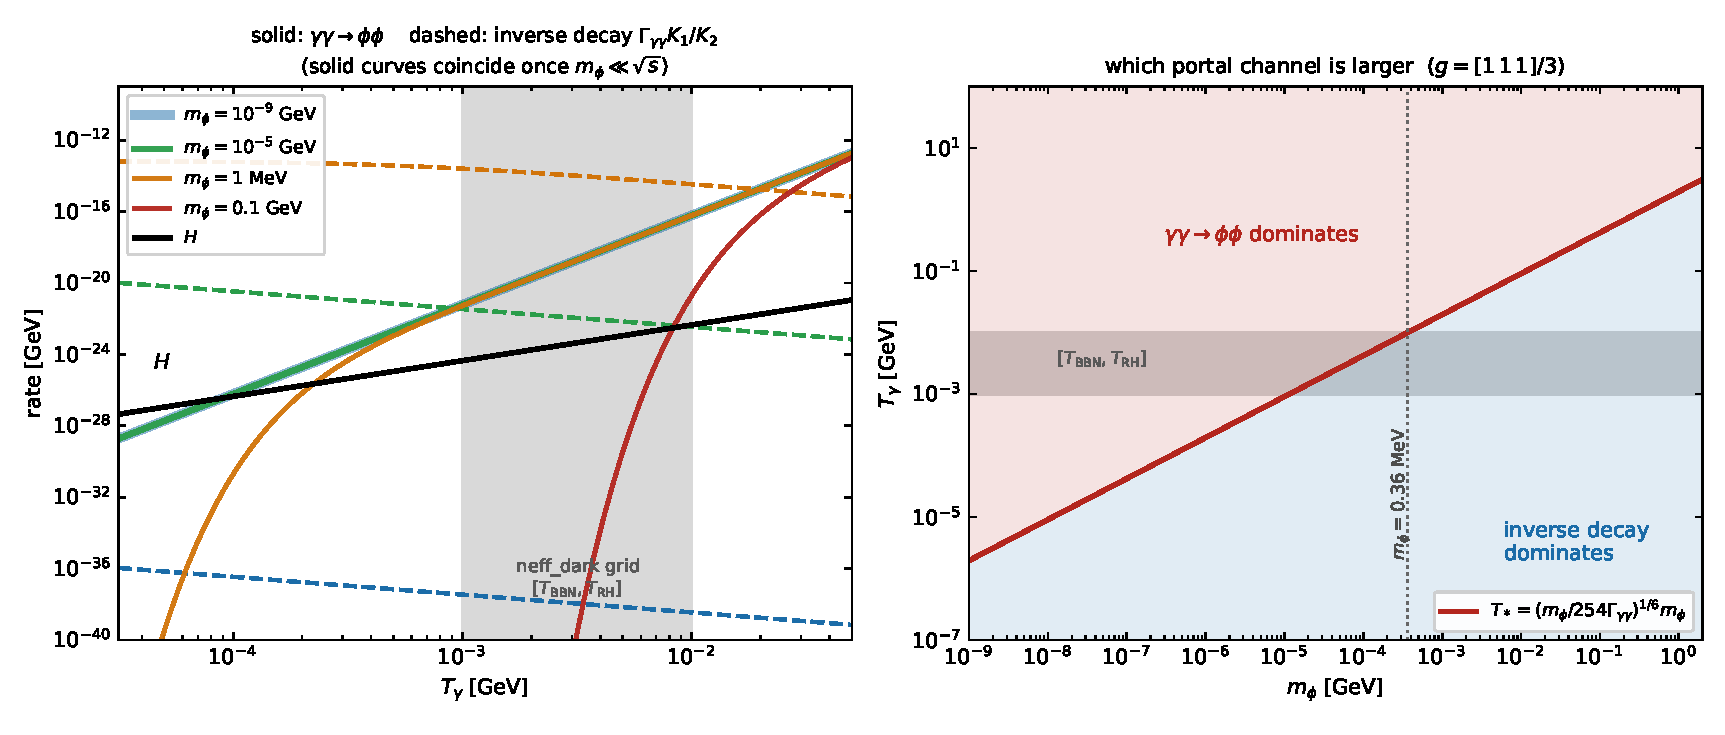
\includegraphics[width=\textwidth]{gg_phiphi_rates.pdf}
\caption{Left: the two portal rates vs.\ $\Tg$ (solid $\gamma\gamma\to\phi\phi$,
dashed $\Ggg K_1/K_2$), with $H$ in black and the \texttt{neff\_dark} grid
$[T_{\rm BBN},T_{\rm RH}]=[1,10]\,$MeV shaded. The solid curves for
$m_\phi=10^{-9}$ and $10^{-5}\,$GeV coincide because $\sigma$ is
$m_\phi$-independent for $s\gg m_\phi^2$. Right: eq.~\eqref{eq:Tstar}.}
\end{figure}

\begin{figure}[h]\centering
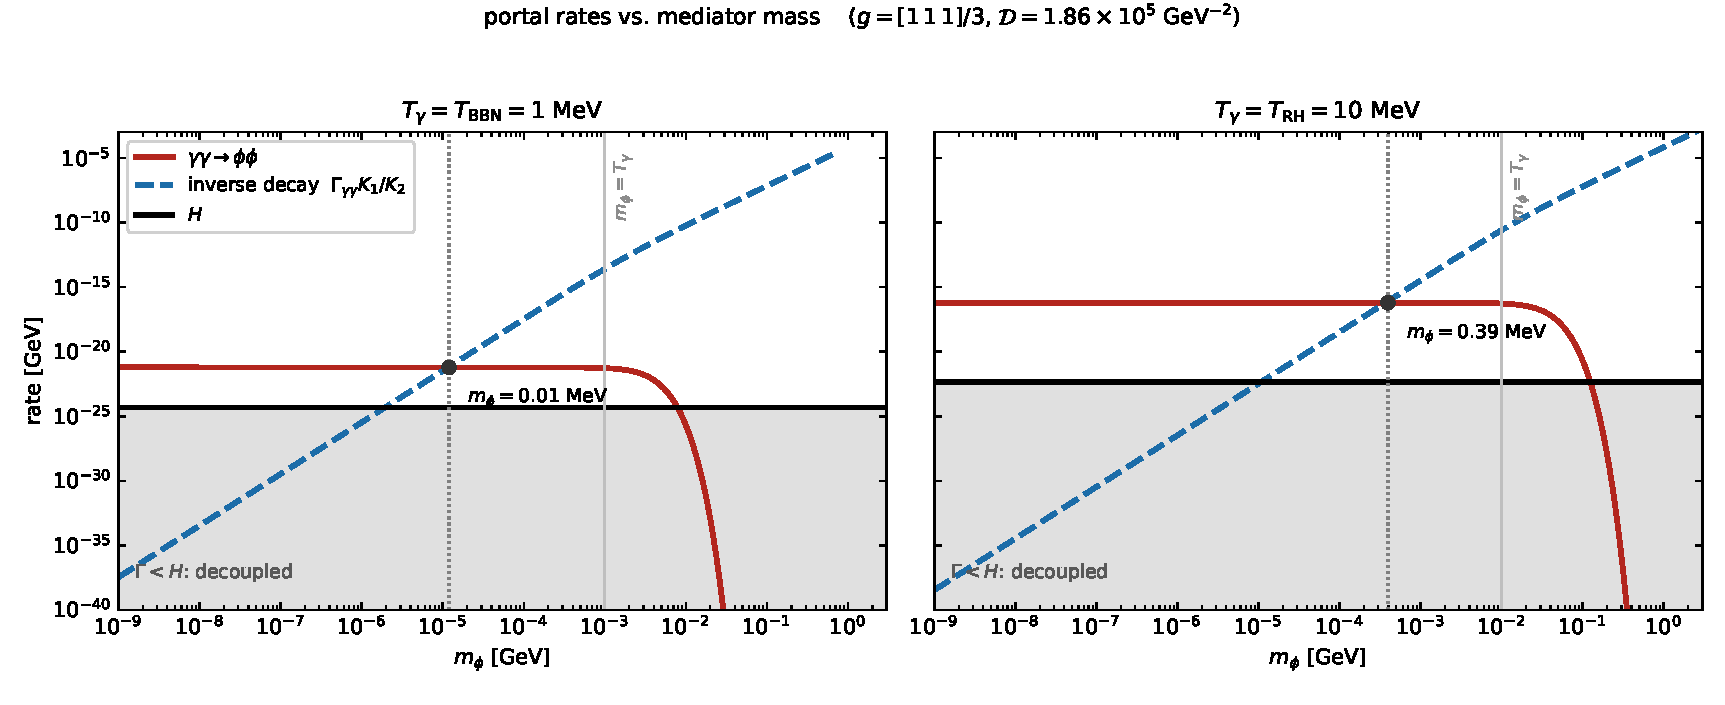
\includegraphics[width=\textwidth]{gg_phiphi_rates_vs_mphi.pdf}
\caption{The same two rates at fixed $\Tg$, as a function of $m_\phi$. Inverse
decay (blue) grows as $m_\phi^3$ through $\Ggg$; $\gamma\gamma\to\phi\phi$ (red)
is flat for $m_\phi\ll\Tg$ --- $g_{\phi\gamma\gamma}$ carries no $m_\phi$ --- and
cuts off by threshold above $m_\phi\sim\Tg$. They cross at $m_\phi=0.01\,$MeV
($\Tg=1\,$MeV) and $0.39\,$MeV ($\Tg=10\,$MeV), the inverse of
eq.~\eqref{eq:Tstar}. Left of those points the code's portal is missing the
dominant channel; note that the red curve stays above $H$ there by three to six
orders of magnitude while the blue one drops below it.}
\end{figure}

On the default grid, with $T_{\rm RH}=10\,$MeV, inverse decay is the larger
channel everywhere only for
%
\begin{equation}
  m_\phi \;>\; (T_{\rm RH}/1.97)^{3/2} = 3.6\times10^{-4}\,\mathrm{GeV}
  = 0.36\,\mathrm{MeV}.
\end{equation}
%
\begin{center}
\begin{tabular}{cccccc}
\hline
$m_\phi$ [GeV] & $\Tg$ [GeV] & $\Ggg K_1/K_2$ & $\Gamma_{\gamma\gamma\to\phi\phi}$
 & ratio & $\Gamma_{\gamma\gamma\to\phi\phi}/H$\\
\hline
$10^{-9}$ & $10^{-2}$ & $3.5\times10^{-39}$ & $6.1\times10^{-17}$ & $1.8\times10^{22}$ & $1.4\times10^{6}$\\
$10^{-5}$ & $10^{-2}$ & $3.5\times10^{-23}$ & $6.1\times10^{-17}$ & $1.8\times10^{6}$  & $1.4\times10^{6}$\\
$10^{-3}$ & $10^{-2}$ & $3.4\times10^{-15}$ & $6.1\times10^{-17}$ & $1.8\times10^{-2}$ & $1.4\times10^{6}$\\
$10^{-1}$ & $10^{-2}$ & $6.0\times10^{-8}$  & $2.0\times10^{-21}$ & $3.3\times10^{-14}$& $4.4\times10^{1}$\\
$1$       & $10^{-2}$ & $6.8\times10^{-5}$  & $\sim10^{-94}$      & $\sim0$            & $\sim0$\\
\hline
\end{tabular}
\end{center}

\paragraph{Consequence (not yet implemented).} At $m_\phi=10^{-9}\,$GeV
\texttt{neff\_dark} currently returns \texttt{never\_coupled}, $\Delta N_{\mathrm{eff}}=0$ for
all but the largest $g_\chi$ (its portal ratio peaks at $7.9\times10^{-14}$ for
$g_\chi=10^{-10}$). Including $\gamma\gamma\to\phi\phi$ gives
$\Gamma/H\simeq1.4\times10^{3}$--$1.4\times10^{6}$ across the grid, so $\phi$ is
thermal at BBN for \emph{every} coupling, $\Delta N_{\mathrm{eff}}\simeq0.571$ (one real scalar
at $T_{\rm dark}=\Tg$) --- the value the code already produces at
$m_\phi=10^{-9}$, $g_\chi=1$. The light-mediator panels would acquire a
coupling-independent $\Delta N_{\mathrm{eff}}$ exclusion.

\end{document}
